% !BIB TS-program = biber
\pdfoutput=1
\pdfminorversion=5

\begingroup\expandafter\expandafter\expandafter\endgroup
\expandafter\ifx\csname pdfsuppresswarningpagegroup\endcsname\relax
\else
  \pdfsuppresswarningpagegroup=1\relax
\fi

\documentclass[11pt]{scrartcl}

\usepackage[letterpaper]{geometry}

\usepackage[version=3]{mhchem} % Formula subscripts using \ce{}, e.g., \ce{H2SO4}
\usepackage{latexsym,amsmath,amssymb}
\usepackage{bm}

\usepackage[utf8]{inputenc}

\usepackage[hyphens]{url}

\usepackage{graphicx}
\usepackage{caption,subcaption}

%\captionsetup[algorithm]{labelformat=empty}

\usepackage{booktabs,multirow}

\usepackage{mathtools}
\usepackage{tablefootnote}

%better printing of numbers
\usepackage[T1]{fontenc}
\usepackage[english]{babel}
\usepackage{csquotes}
\usepackage{textcomp}

\usepackage{authblk}

%cross file reference
\usepackage{xr}
\externaldocument{GPU-integrator-paper}

\usepackage[binary-units]{siunitx}
\sisetup{group-separator={,},
     detect-all,
     binary-units,
     list-units = single,
     range-units = single,
     range-phrase = --,
     per-mode = symbol-or-fraction,
     separate-uncertainty = true,
     multi-part-units = single,
     list-final-separator = {, and }
%    scientific-notation = fixed
}

\DeclareSIUnit\atm{atm}


\usepackage{doi}
\usepackage[backend=biber,
            hyperref=true,
            autolang=hyphen,
            style=numeric-comp,
            bibencoding=UTF-8,
            giveninits=true,
            maxbibnames=1000,
            terseinits=true,
            block=none,
            sorting=none
]{biblatex}

\hypersetup{linkcolor=blue, citecolor=blue, colorlinks=true}

% biblatex
\addbibresource{GPU-integrator-paper.bib}

% remove "in: " from articles
\renewbibmacro{in:}{%
  \ifentrytype{article}{}{%
  \printtext{\bibstring{in}\intitlepunct}}
}

\graphicspath{{./figures/}}

\title{Supplementary material for ``An investigation of GPU-based stiff chemical kinetics integration methods''}

\author[1]{Nicholas~J.\ Curtis\thanks{Email: \href{mailto:nicholas.curtis@uconn.edu}{nicholas.curtis@uconn.edu}}}
\author[2]{Kyle~E.\ Niemeyer}
\author[1]{Chih-Jen Sung}

\affil[1]{Department of Mechanical Engineering, University of Connecticut, Storrs, CT, USA}
\affil[2]{School of Mechanical, Industrial, and Manufacturing Engineering, Oregon State University, Corvallis, OR, USA}

\date{}


\begin{document}
\maketitle

%%%%%%%%%%%%%%%%%%%%%%%%%%%%%%%%%%%%%
\section{Raw performance plots}
%%%%%%%%%%%%%%%%%%%%%%%%%%%%%%%%%%%%%
\label{S:raw}

In this section we present the plots of the raw, unnormalized performance data for completeness, as described in Sec.~\ref{S:results}.
Figures~\ref{F:raw_perf_H2CO} and \ref{F:raw_perf_CH4} show performance for the hydrogen and GRI-Mech 3.0 models, respectively.

\begin{figure}[htbp]
  \centering
  \begin{subfigure}{0.49\textwidth}
      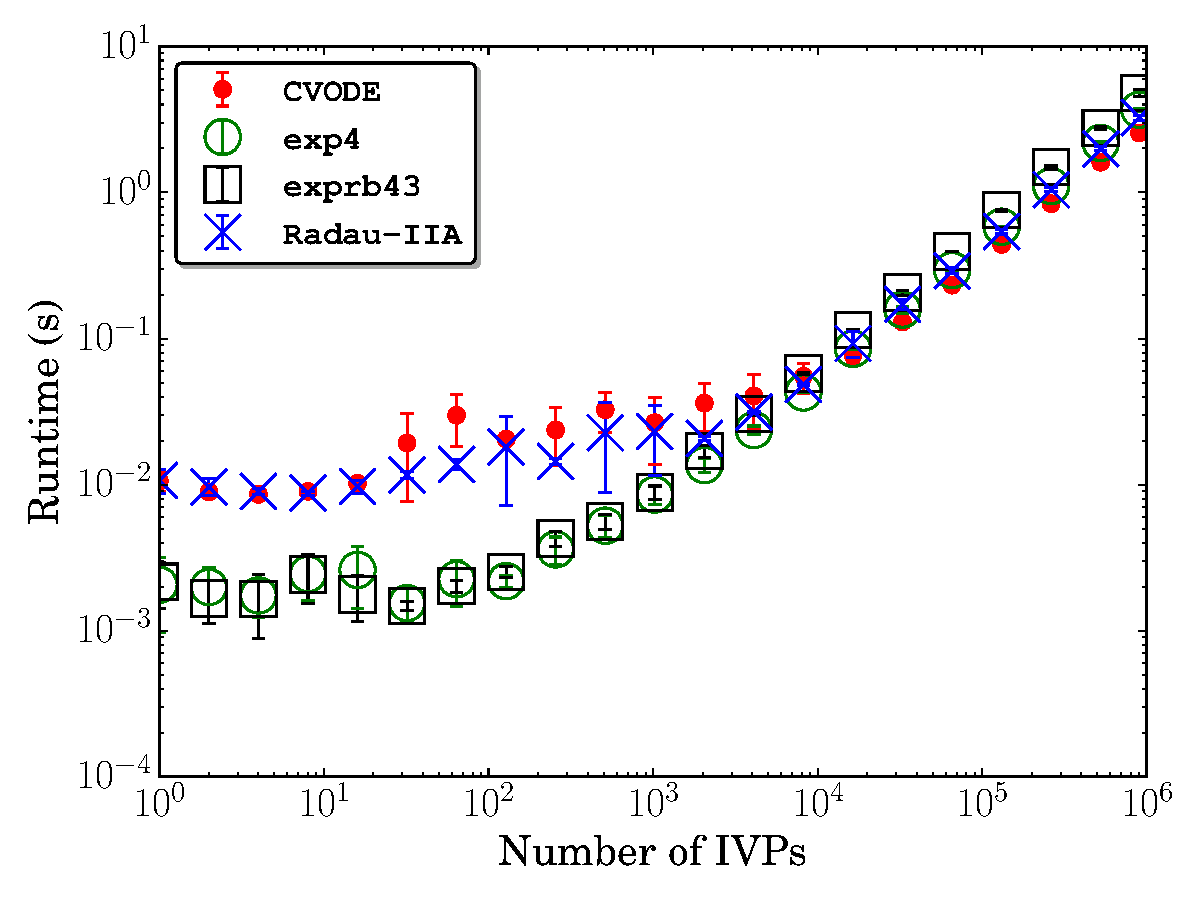
\includegraphics[width=\linewidth]{H2_1e-06_cpu_nonorm.pdf}
      \caption{CPU performance results for $\Delta t = \SI{e-6}{\second}$}
  \end{subfigure}
  %\hfill
  \begin{subfigure}{0.49\textwidth}
      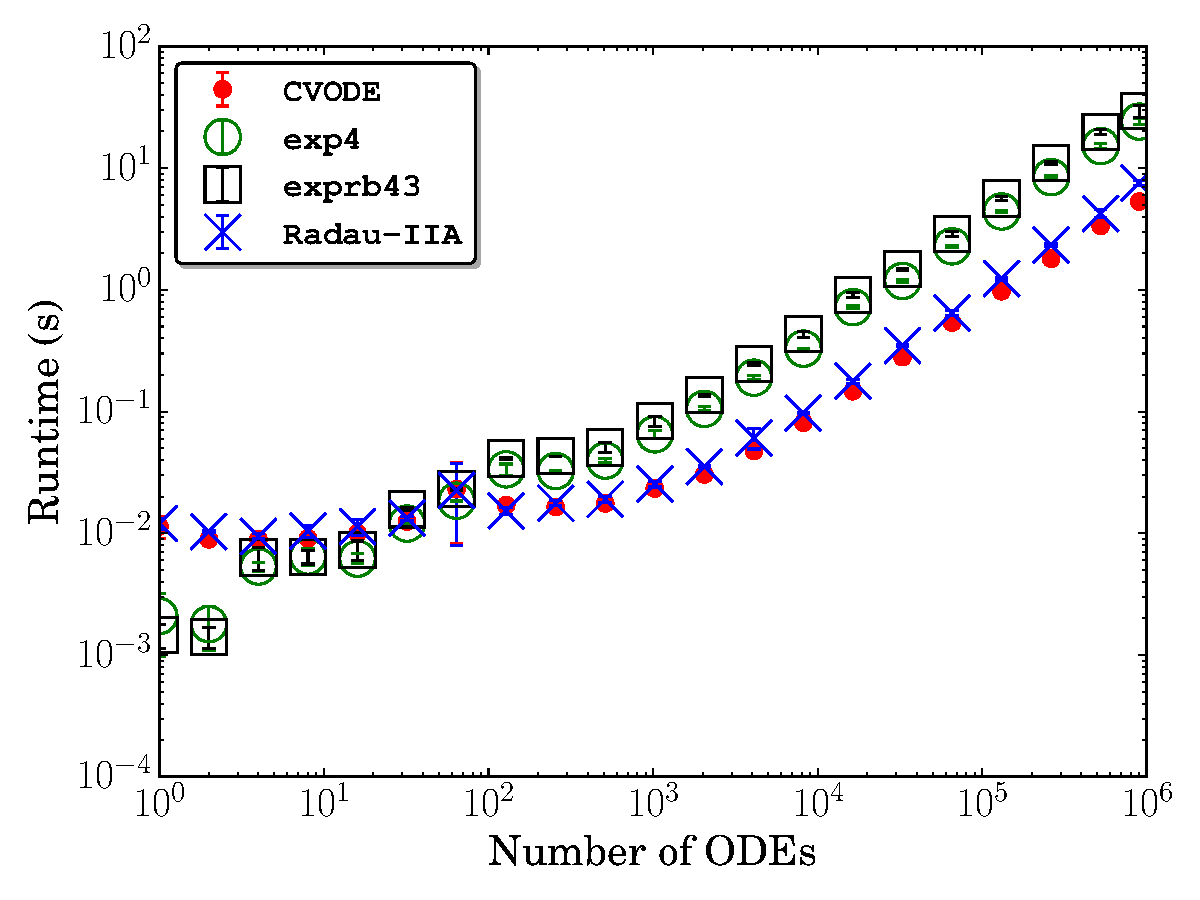
\includegraphics[width=\linewidth]{H2_1e-04_cpu_nonorm.pdf}
      \caption{CPU performance results for $\Delta t = \SI{e-4}{\second}$}
  \end{subfigure}\\
  \begin{subfigure}{0.49\textwidth}
      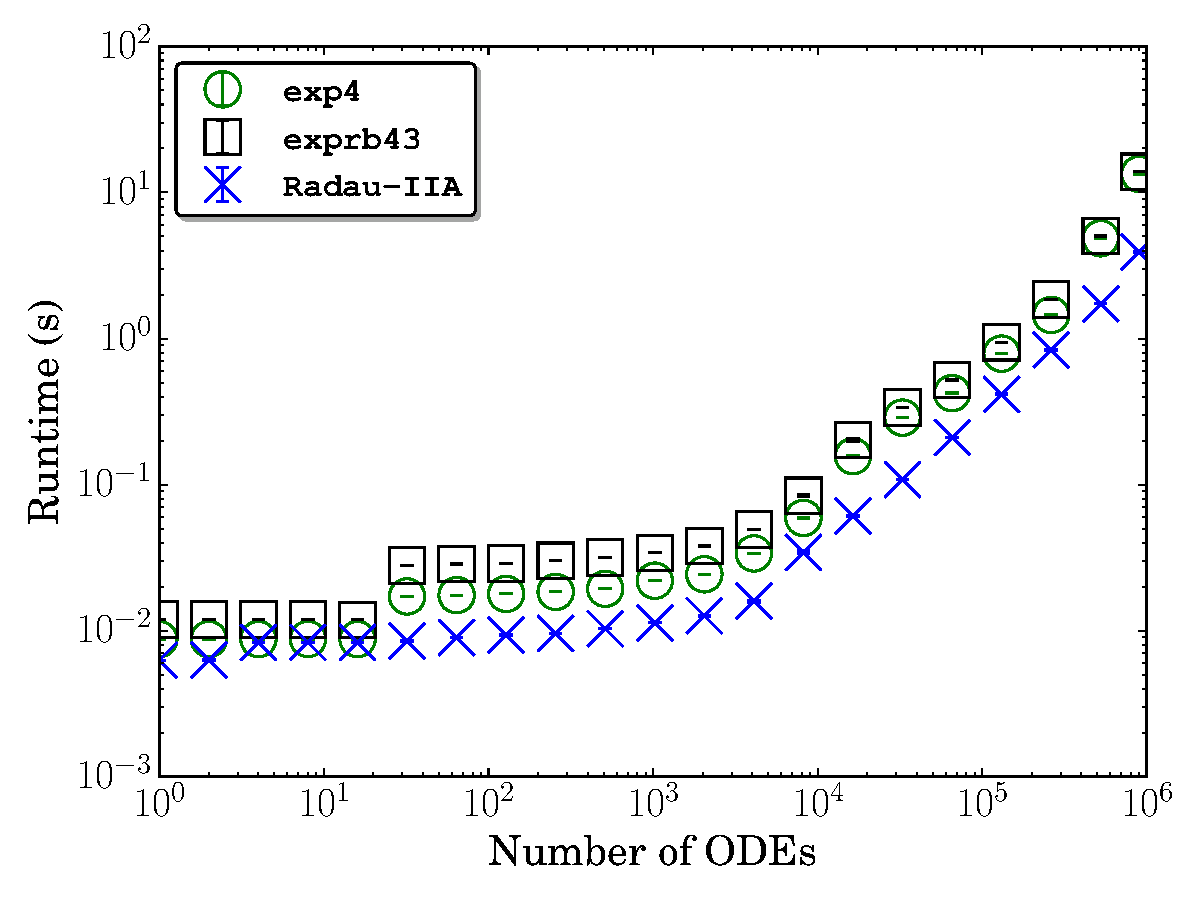
\includegraphics[width=\linewidth]{H2_1e-06_gpu_nonorm.pdf}
      \caption{GPU performance results for $\Delta t = \SI{e-6}{\second}$}
  \end{subfigure}
  %\hfill
  \begin{subfigure}{0.49\textwidth}
      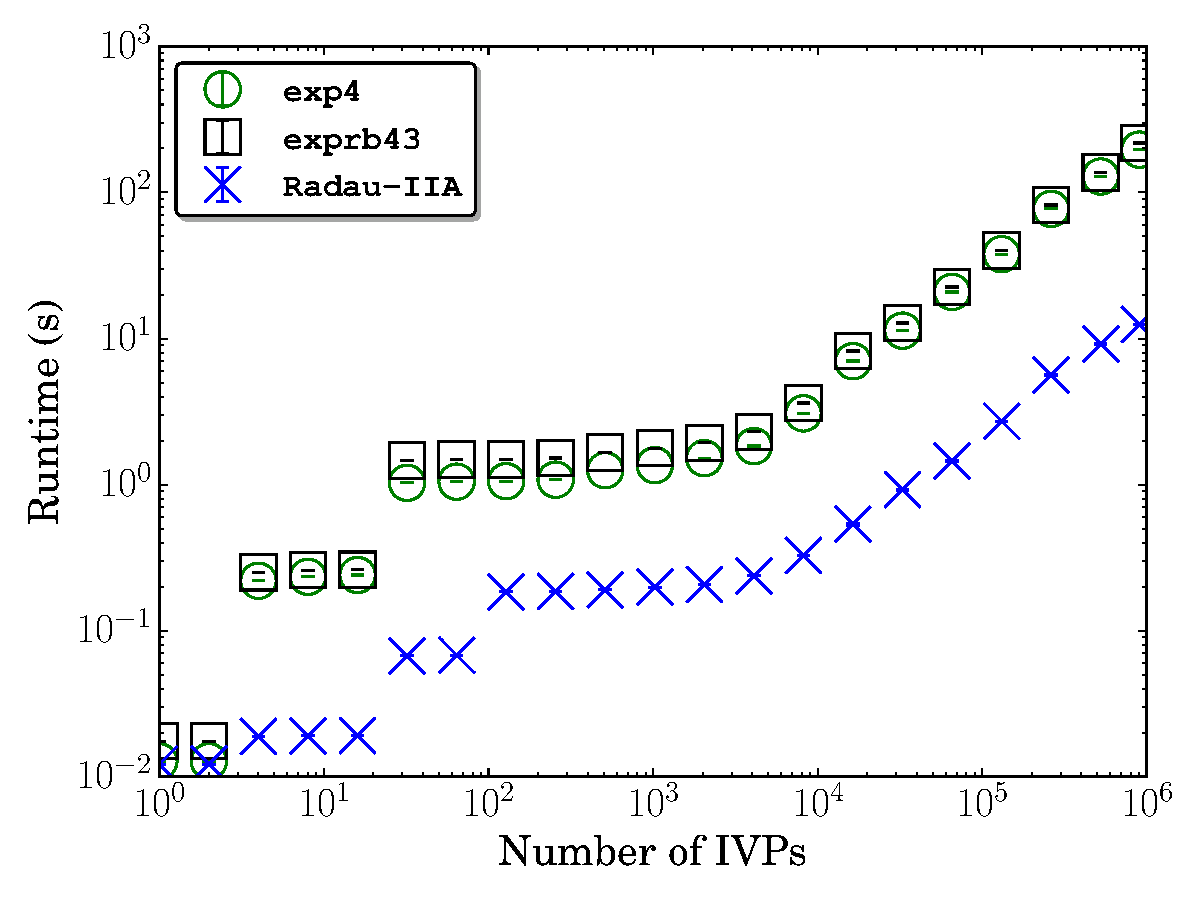
\includegraphics[width=\linewidth]{H2_1e-04_gpu_nonorm.pdf}
      \caption{GPU performance results for $\Delta t = \SI{e-4}{\second}$}
  \end{subfigure}
  \caption{Average (unnormalized) runtimes of the integrators on the CPU and GPU for the hydrogen model at two different global time-step sizes.
  Error bars indicate standard deviation.
  Data, plotting scripts, and figure files available under CC-BY~\cite{paperscript:2017}.}
  \label{F:raw_perf_H2CO}
\end{figure}

\begin{figure}[htbp]
  \centering
  \begin{subfigure}{0.49\textwidth}
      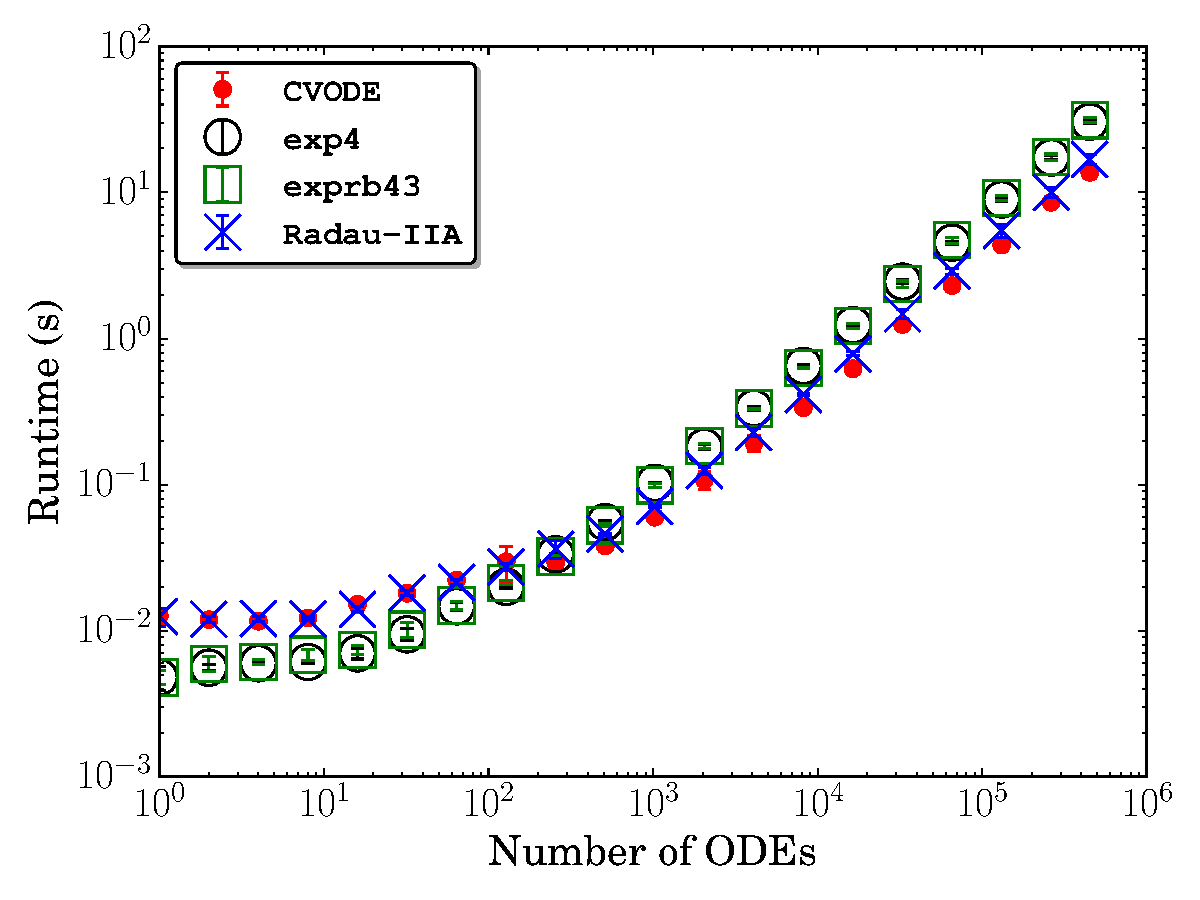
\includegraphics[width=\linewidth]{CH4_1e-06_cpu_nonorm.pdf}
      \caption{CPU performance results for $\Delta t = \SI{e-6}{\second}$}
  \end{subfigure}
  %\hfill
  \begin{subfigure}{0.49\textwidth}
      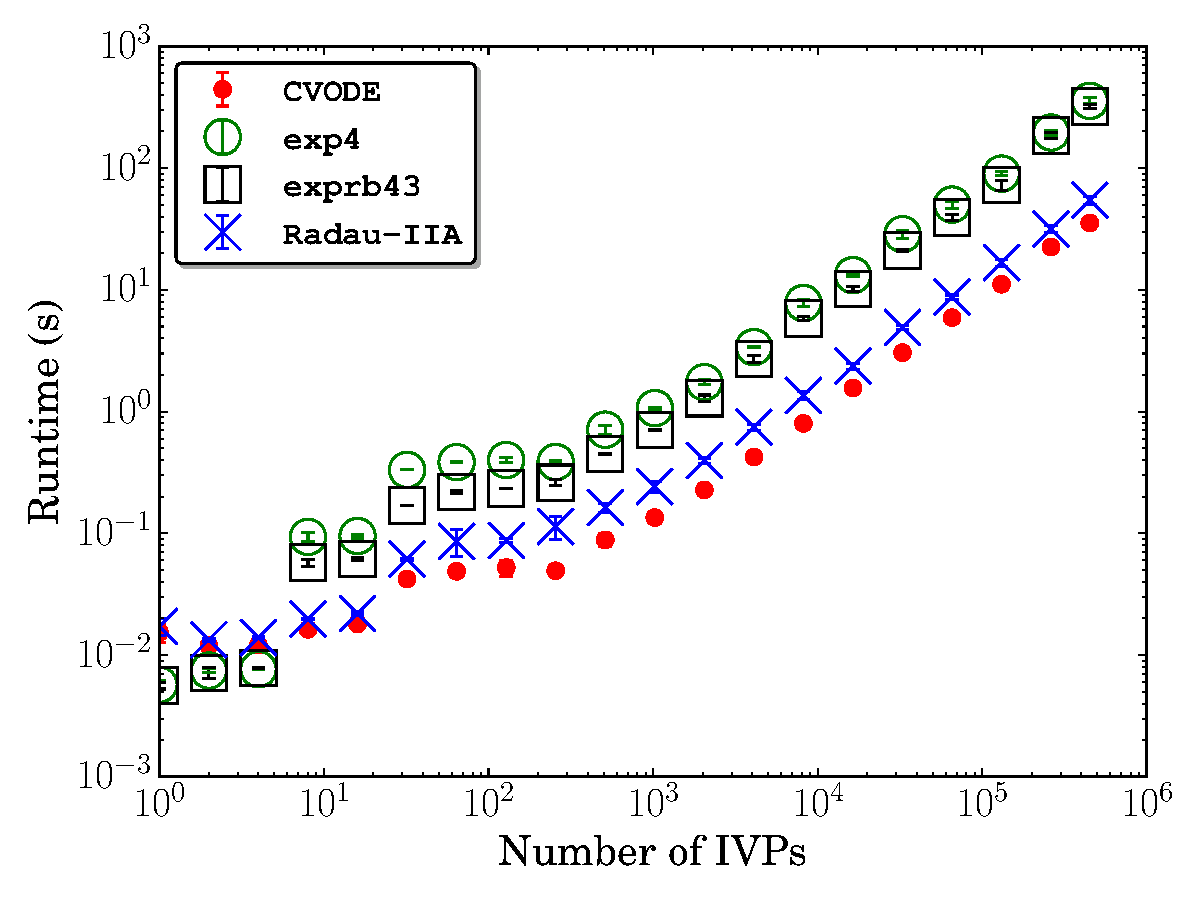
\includegraphics[width=\linewidth]{CH4_1e-04_cpu_nonorm.pdf}
      \caption{CPU performance results for $\Delta t = \SI{e-4}{\second}$}
  \end{subfigure}\\
  \begin{subfigure}{0.49\textwidth}
      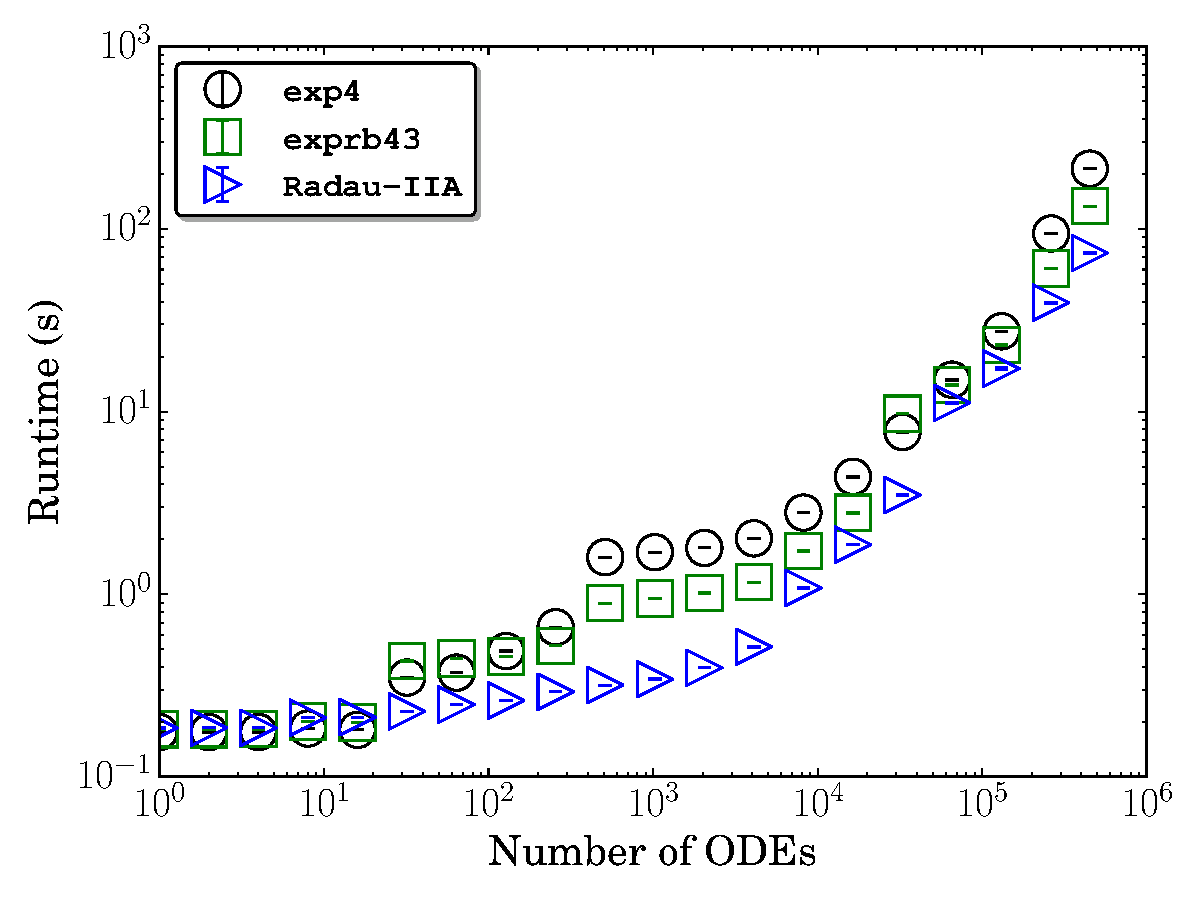
\includegraphics[width=\linewidth]{CH4_1e-06_gpu_nonorm.pdf}
      \caption{GPU performance results for $\Delta t = \SI{e-6}{\second}$}
  \end{subfigure}
  %\hfill
  \begin{subfigure}{0.49\textwidth}
      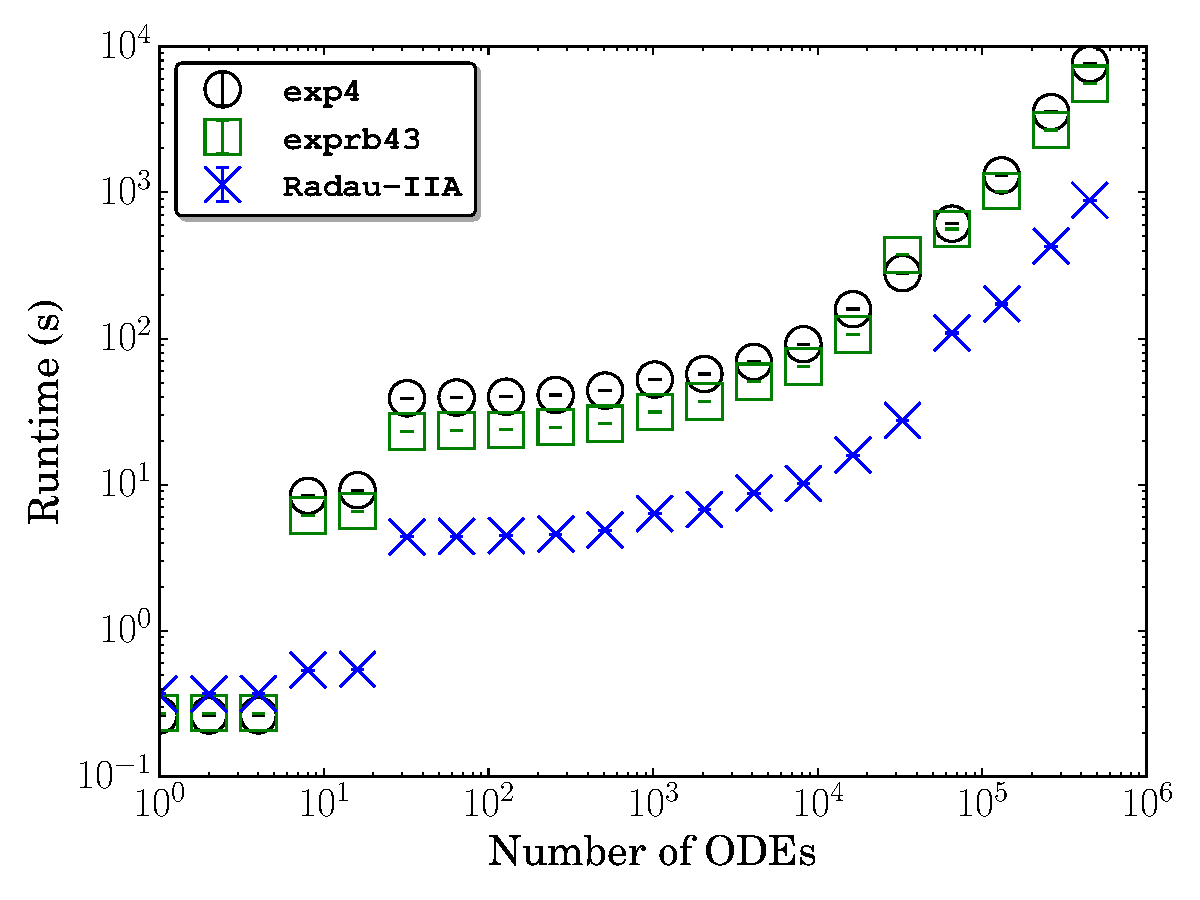
\includegraphics[width=\linewidth]{CH4_1e-04_gpu_nonorm.pdf}
      \caption{GPU performance results for $\Delta t = \SI{e-4}{\second}$}
  \end{subfigure}
  \caption{Average (unnormalized) runtimes of the integrators on the CPU\slash GPU for the GRI-Mech 3.0 model at two different global time-step sizes.
  Error bars indicate standard deviation.
  Data, plotting scripts, and figure files available under CC-BY~\cite{paperscript:2017}.}
  \label{F:raw_perf_CH4}
\end{figure}

\clearpage

\section{Characterization of partially stirred reactor data}
\label{S:pasr_charac}

\begin{figure}[htbp]
  \centering
  \begin{subfigure}{0.48\textwidth}
      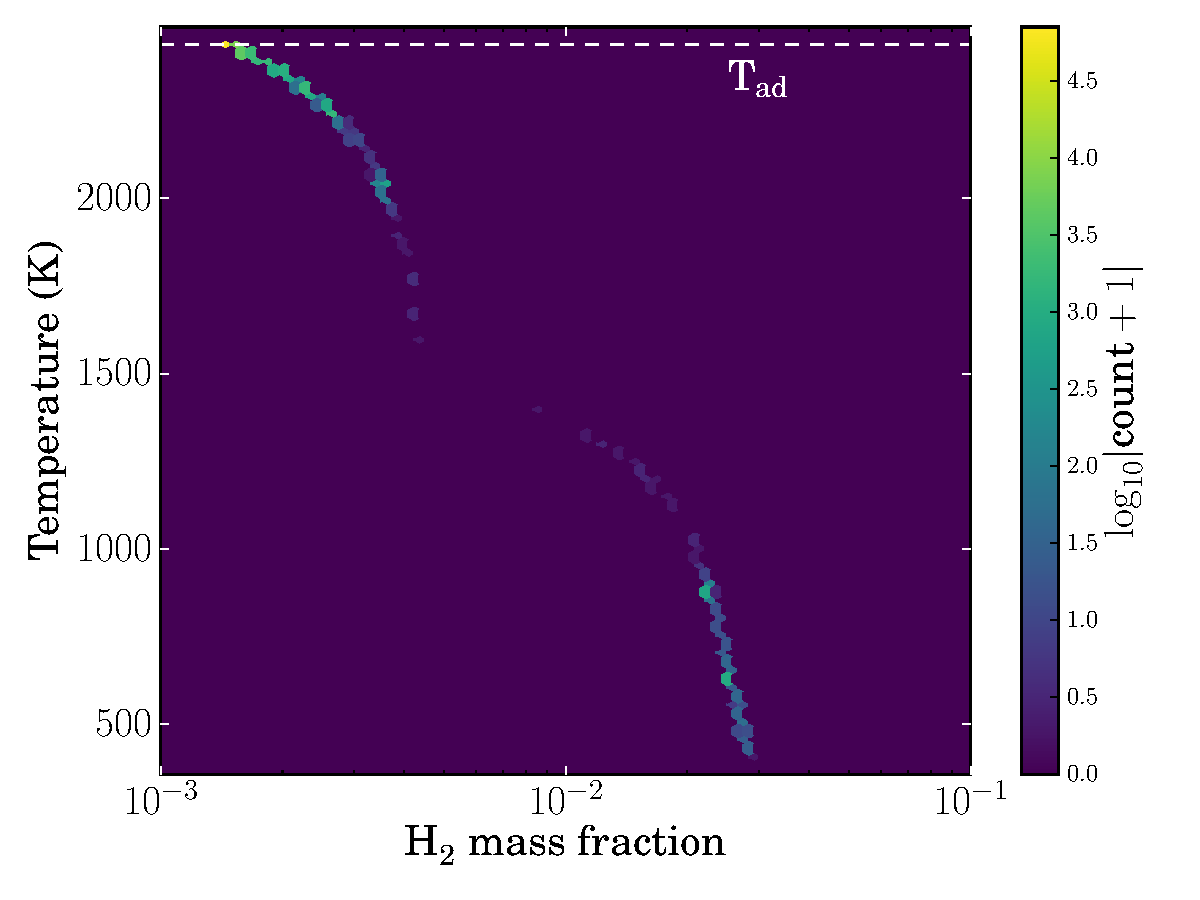
\includegraphics[width=\linewidth]{H2_pasr_dist.pdf}
      \caption{Temperature\slash \ce{H2} mass fraction distribution for a hydrogen run.}
  \end{subfigure}
  \hfill
  \begin{subfigure}{0.48\textwidth}
      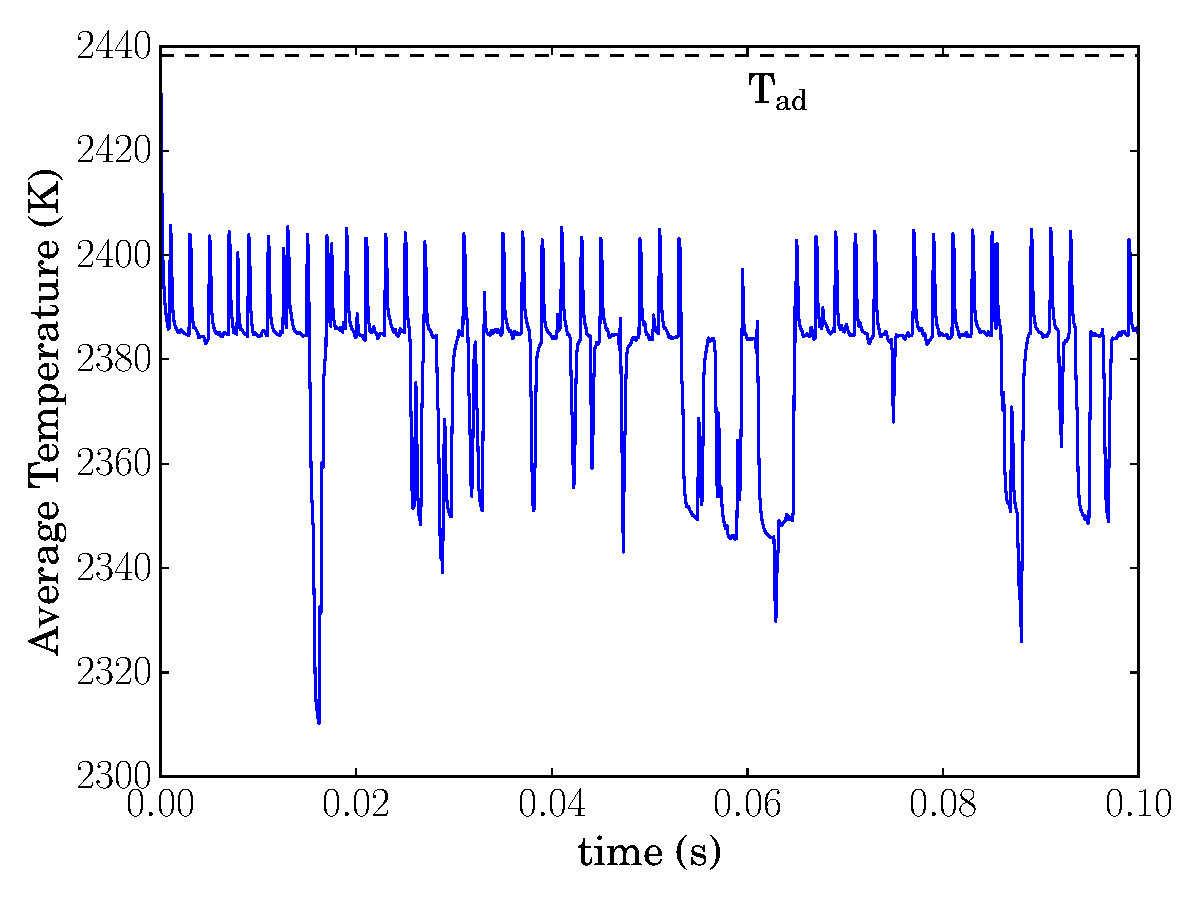
\includegraphics[width=\linewidth]{H2_pasr_tbar.pdf}
      \caption{Average temperature in the PaSR for hydrogen run.}
  \end{subfigure}\\
  \begin{subfigure}{0.48\textwidth}
      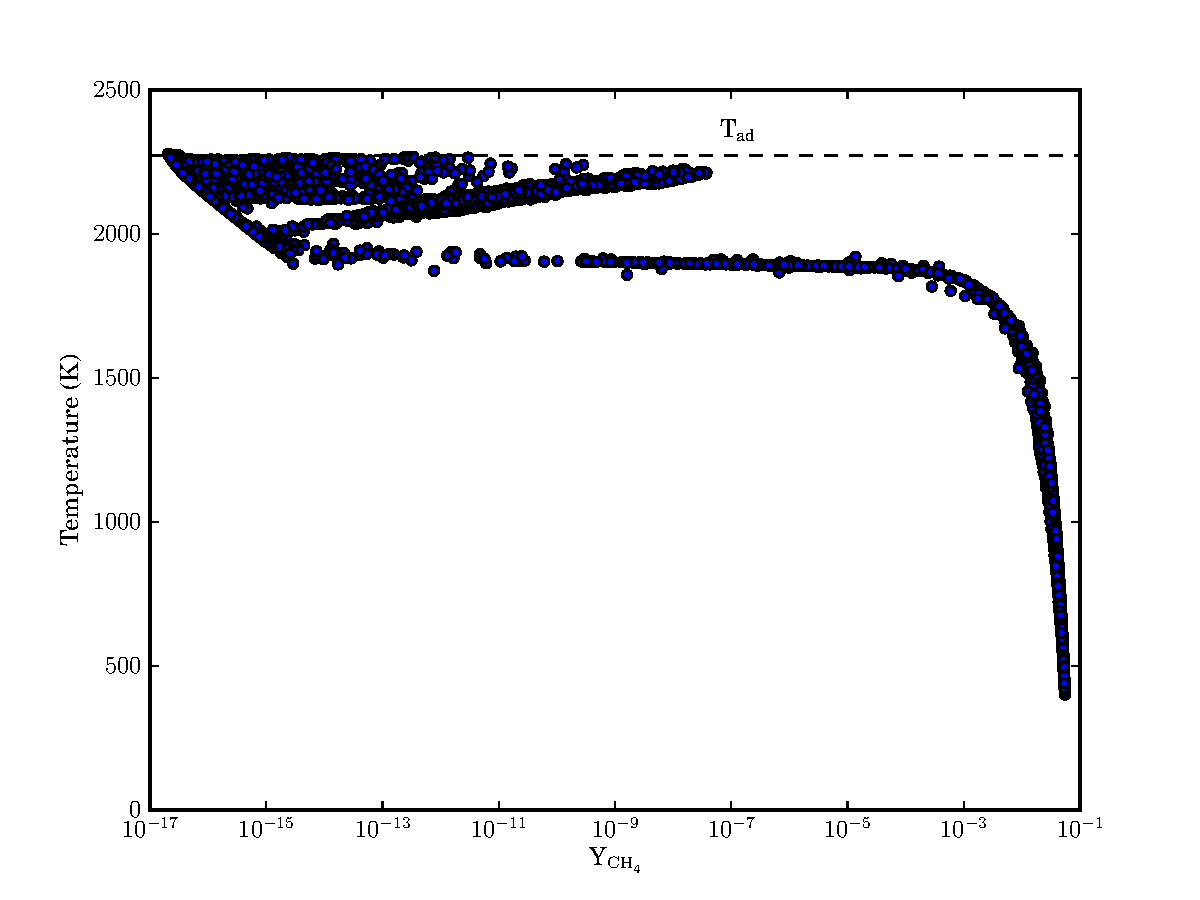
\includegraphics[width=\linewidth]{CH4_pasr_dist.pdf}
      \caption{Temperature\slash \ce{CH4} mass fraction distribution for a GRI-Mech 3.0 run.}
  \end{subfigure}
  \hfill
  \begin{subfigure}{0.48\textwidth}
      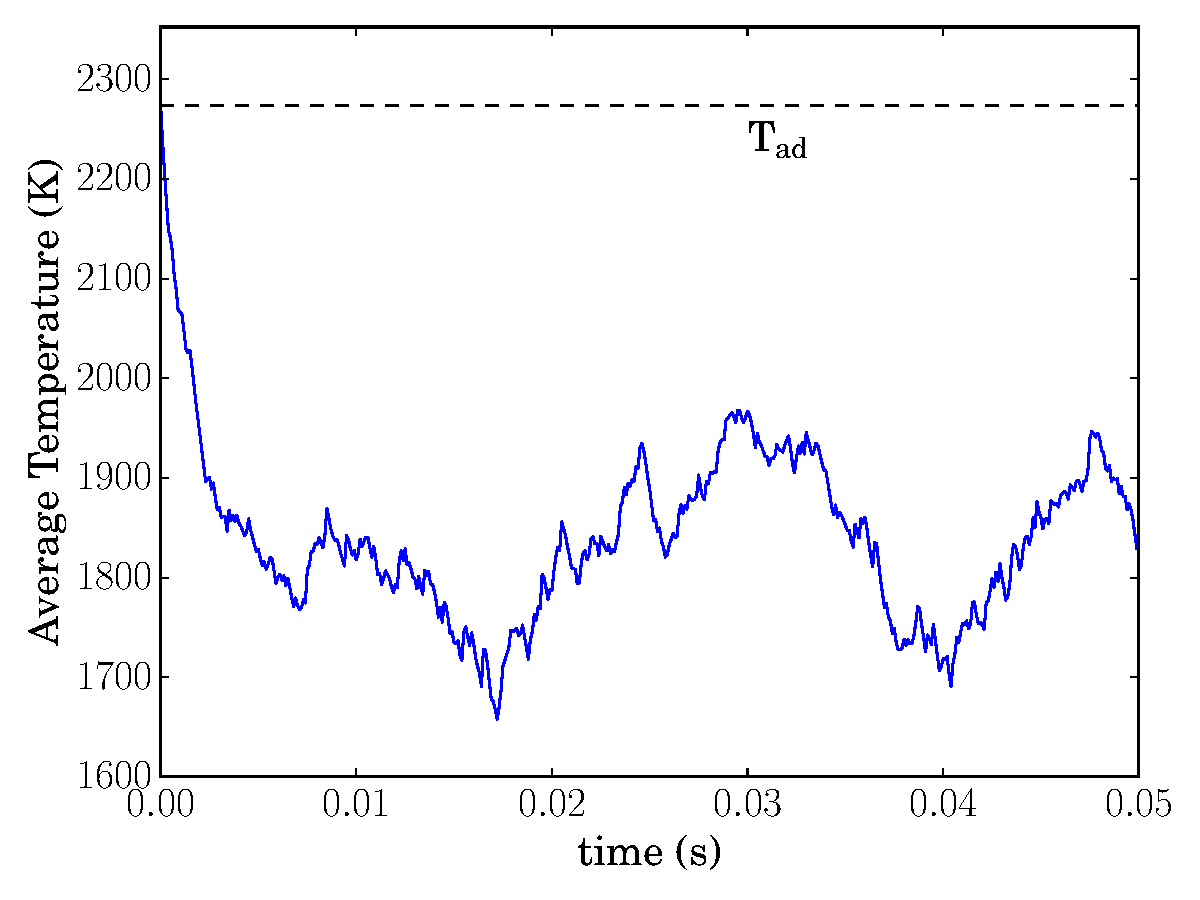
\includegraphics[width=\linewidth]{CH4_pasr_tbar.pdf}
      \caption{Average temperature in the PaSR for a GRI-Mech 3.0 run.}
  \end{subfigure}
  \caption{Characterizations of the conditions sampled from the PaSR at \SI{400}{\kelvin}, \SI{1}{\atm} for both models.
  The adiabatic flame temperature $\text{T}_{\text{ad}}$ is by a dashed line in all cases.
  Data, plotting scripts, and figure files available under CC-BY~\cite{paperscript:2017}.}
  \label{F:pasr_characterization}
\end{figure}

Figure~\ref{F:pasr_characterization} shows a characterization example of the PaSR conditions sampled for validation and performance testing in this work; a wide range of temperatures and fuel-mass fractions are observed for both models.
Significantly more diversity in fuel mass-fraction is seen for the GRI-Mech 3.0 near the adiabatic flame temperature.
Further, the hydrogen model is more sensitive to the mixing\slash pairing time-scales, showing many large temperature changes quickly recovering to a semi-stable temperature.
The databases used in this work are available online~\cite{Curtis2016:h2,Curtis2016:ch4}.


\printbibliography[title={References}]

\end{document}
